\documentclass{article}

\usepackage{graphicx}
\usepackage{hyperref}
\usepackage{amssymb}

\title{Yelp and Crime}  % TODO
\author{Kenneth Lin, Sid Naik, Tom McCormick}
\date{\today}

\renewcommand{\labelitemi}{\checkmark}

\begin{document}
\maketitle

\section{Problem Statement and Background}

For our CS 194 final project, we decided to investigate the potential
relationship between the City of San Francisco public safety data set and
the data set provided by the Yelp API. With the recent civil unrest both
inside and outside of the United States, and more recently, right here in
Berkeley, we thought that it would be interesting to look into the factors
that promote crime. One of our team members (Kenneth Lin) had also been
robbed recently, so the problem is one that is dear to our hearts. Perhaps
the most well-known correlation with crime rate is the income level of a
neighborhood -- the lower the income level, the higher the crime rate
\cite[p.93-94]{levitt-the-changing-relationship}. However, we wanted to
show something more interesting. In particular, Yelp restaurants, in our
experience, often reflect the wealth and well-being of its surrounding
neighborhood -- the presence of many highly rated restaurants, we believed,
reflect the optimism in the economy of a neighborhood, as well as the
wealth and ``goodness'' of that neighborhood. Therefore, we had conjectured
that crime would negatively impact restaurant ratings, or that low
restaurant ratings would be correlated with areas of high crime. We worked
to show this throughout our project.

% At first, we explored each data set individually to discover general
% patterns in the data set. After that, we delved into our main problem. We
% are interested in the relationship (if any) between the quality of
% restaurants and the frequency and severity of crime. In particular, we
% wanted to know

In particular, we wanted to know

\begin{itemize}
\item the effect of crime on restaurant ratings (or vice versa)
\item the distribution of crime vs. the distribution of ratings
\end{itemize}

We had also wanted to predict crime density / severity using restaurant
ratings or vice versa, but along the way we ran into issues of determining
or implying causation in any of the methods we used. By using one to
predict the other and trying to draw useful conclusions from this, we run
the risk of assuming causation without definitive proof. There are many
other problems that may arise as a result of this, which will be discussed
in the \textbf{\nameref{sec:lessons-learned}} section.

\subsection{City of San Francisco Public Safety Data Set}

The City of San Francisco public safety dataset is a record, written by the
San Francisco Police Department, of incoming incident reports, either via
phone call, in person, or otherwise. The incidents are reported via the
SFPD CABLE crime incident reporting system. The incidents are reported over
the course of more than 11 years, from 1/1/2003 to present. A sample of
records in the dataset looks like the following:

\begin{center}
  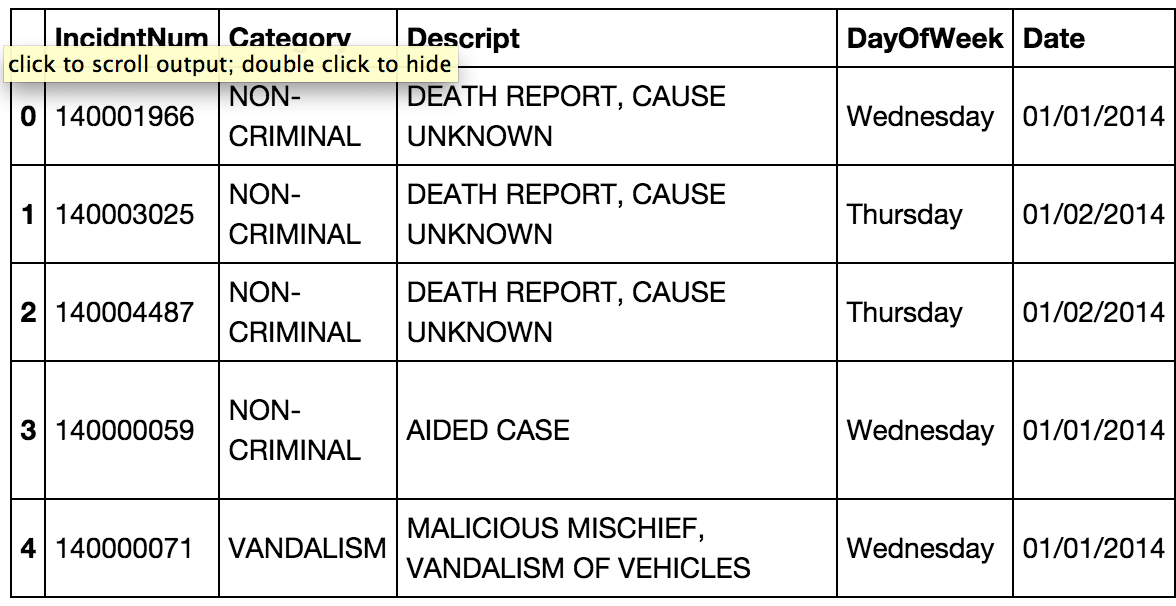
\includegraphics[scale=0.5]{sf_city_sample_1.png} \\
  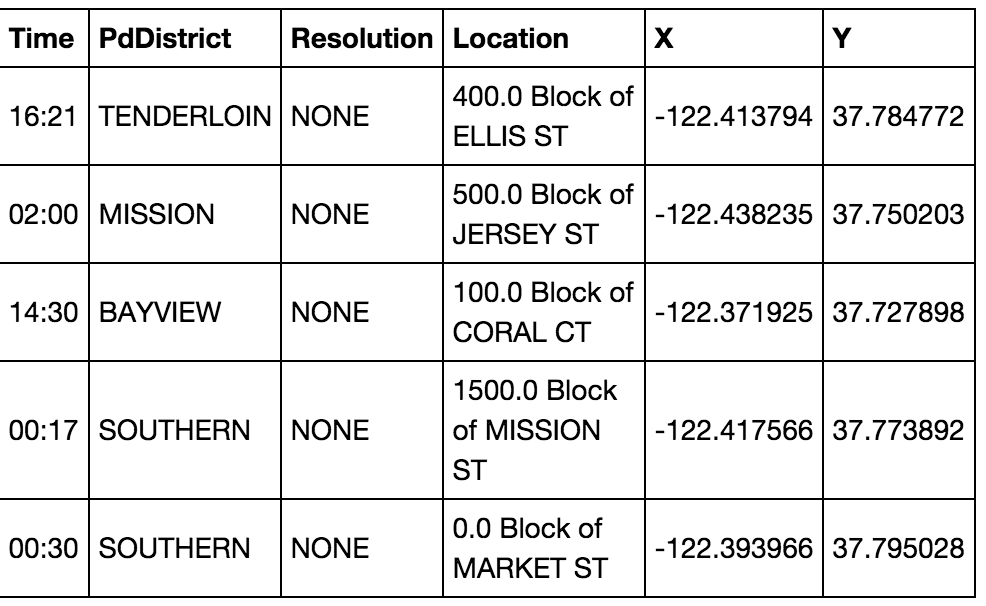
\includegraphics[scale=0.5]{sf_city_sample_2.png} \\
  Figure 1: Sample of San Francisco crime data set
\end{center}

-- introduction of data set
-- collection conditions

The majority of the fields are self-explanatory. However, there are a few
things to note:
\begin{enumerate}
\item Category and descript are both categories, but category is more
  general. There are only 36 different ``Categories'' while there are 499
  different ``Descript''s in the year of 2014.
\item Resolution, though none are shown in the sample above, denote whether
  any action was taken and what that action was.
\item X denotes longitude, while Y denote latitude.
\end{enumerate}

A more detailed analysis is in the attached \texttt{analysis.ipynb}.

\subsection{Yelp Data Set}

Yelp.com is a platform which publishes crowd-sourced reviews about local
businesses. On Yelp, customers who have used the services of local
businesses may write reviews of these businesses and provide ratings of
their satisfaction. Reviewers may select from between 1 to 5 stars for each
review they make, and a business's average rating is the average of the
ratings of each of the reviews it has received. Yelp supplies a platform
for all kinds of local businesses ranging from restaurants to barbers to
museums; however, for the purpose of our research, we will look primarily
at restaurants as they are a very large majority of the reviews on Yelp.

There are two primary ways to access the data on Yelp. First, we can
utilize the search / business API
(\url{http://www.yelp.com/developers/documentation}). The search / business
API provides a way to search for local businesses matching a particular key
term (``restaurants'', for example) near a geographical location, and get
all the rating / review information about that restaurant. The API further
allows us to narrow the search to only the geographically closest
restaurants (not ranked by rating). This gives us a way to link the
geographical location of crime incidents to the types of restaurants near
that incident.

The other way of accessing Yelp data is through the academic data set
(\url{https://www.yelp.com/academic_dataset}). The Yelp academic data set
provides all the data and associated reviews of the 250 closest businesses
for 30 universities, including UC Berkeley. Although not a random sample of
all businesses on Yelp, the academic data set provides a much better
estimate of all businesses in the Yelp data set population.

-- introduction of Yelp
-- two APIs
-- basic analysis

\section{Methods}

\section{Tools}

\section{Results}

\subsection{Putting it together}

-- distribution
-- ratings

-- CONCLUSIONS??!?

-- map visualization problems
---- yelp data biased to near crime
---- not enough data on all of san francisco to create proper viz

-- condition tests in certain neighborhoods

\section{Lessons Learned}
\label{sec:lessons-learned}

\bibliographystyle{IEEEtran}
\bibliography{writeup-bibliography}

\end{document}
